\documentclass[10pt]{article}

\usepackage{graphicx}
\usepackage{amsmath}
\usepackage{amssymb}
\usepackage{braket}
\usepackage{parskip}
\graphicspath{{../../figs/}}

\begin{document}

\title{Hiddem Markov Models for Protein Dynamics}
\maketitle

\section{Motivation}

Traditionally, we have clustered conformation-space into many discrete
voronoi cells and used this clustering to build a large transition matrix.
This results in implied timescales that are consistently faster than they
should be. 

The motivation of this work can be found in considering a simple, two-well,
1D potential. What is the optimal clustering? There are only two physically
stable states, but if we used two \textit{hard} states, conformations on the cusp
of the barrier are considered to be the same as conformations at the bottom of the well.
If the particle moving under this potential diffuses for a bit at the top of the potential,
crossing the line that distinguishes our two hard states, it generates many counts, distorting
the dynamics. 

\begin{figure}[htbp!]
	\centering
	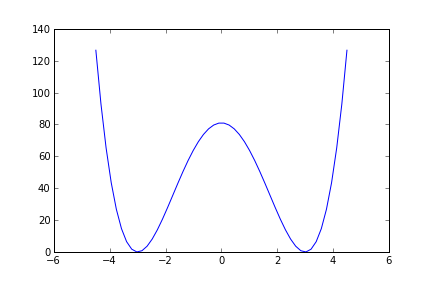
\includegraphics[width=0.8\textwidth]{two-well.png}
	\caption{A two-well potential (blue) and its stationary distribution (green).
	A traditional MSM will produce a discretized approximation (red) to the true stationary
	distribution.}
	\label{two-well}
\end{figure}

The theoretical underpinnings of Markov State Models is that they are used to estimate
the propagator. The true propagator is continuous in $\mathbb{R}^{6N}$, and the typical
approach is to use indicator basis functions to approximate it. This gives step-like
eigenfunctions whose resolution increases with increasing number of states---see
figure \ref{two-well}, red line.  One can imagine
using a different basis set instead. Two Gaussian functions, for example, could describe
dynamics on this potential much better than even a high number of step functions with
many fewer parameters.



\section{HMMs and Baum-Welch}

Deriving a transition matrix from non-overlapping hard states is trivial: for lag time
$\tau$, if the conformation moves from state $i$ to state $j$, we increment the entry
in the count matrix, $C_{ij}$. The transition matrix is a row-stochastic normalization of
this count matrix.

It is impossible to define counts in this way for \textit{fuzzy} states. One might
imagine describing a point at time $t$ not simply as belonging to state $i$, but rather as 
having a vector of memberships $\mathbf{m}$ in each fuzzy state. One might think
that you can get the transition matrix by summing the outer product between each
time-pair of membership vectors as in REF

\begin{equation}
\sum \Ket{\mathbf{m}_t} \Bra{\mathbf{m}_{t+1}}
\end{equation}

This works for the case of quantized memberships, but creates
arbitrarily small transition probabilities due to the multiplication
of many numbers that are less than one. In fact, the problem
of coming up with a transition matrix from fuzzy states is non-trivial.
Going back to our two well potential, consider a conformation sitting at
the top of the barrier. It has membership vector $\mathbf{m}_0 = (0.5,0.5)$. 
After one time step, it is in the same place, $\mathbf{m}_1 =(0.5, 0.5)$
What is the proper transition matrix? Is it the identity matrix? Is it
$frac{1}{4}$ in each position? It's difficult to say.

We require a learning algorithm that can infer from entire trajectories, probable
state definitions and the paths through those states.


Instead of treating the system as a Markov model, we can consider it a Hidden
Markov Model (HMM). The conformation
at a particular time is the observed quantity, or \textit{emission}, and the small number of
(potentially metastable) states
are the hidden states of the model. 

The Baum-Welch algorithm is a particular expectation-maximization (EM) algorithm to simultaneously
learn the parameters of the hidden states (`emission distributions') as well as the rates of transition
through those states (the hidden transition matrix)

\section{Methods}

The Baum-Welch algorithm can only find local maxima in likelihood. It is important to seed
the algorithm with initial transition matrices and state definitions that are close to the
actual ones. In our approach, we use standard gaussian mixture modelling from the scikit-learn
package to define initial gaussian emission distributions. From this density based
approach, we can calculate the BIC of the mixture model to determine the best number of states.
Each conformation is assigned membership values (zero to one) in each gaussian state. As a first approximation
for calculating the transition matrix, conformations are assigned to the state in which their membership
is highest. A normal (relatively few-state) MSM is built from these assignments, and this transition
matrix is used to seed the Baum-Welch algorithm.

After the initial guesses for state definition and transition matrix have been made, the algorithm,
as implemented in the General HMM (ghmm) package for C/python
is run on a set of trajectories. Optimized parameters for the emission distributions and
hidden transition matrix are returned.

There is probably some math to extract the eigenvector/values from this hidden transition matrix.

\begin{subequations}
\begin{align}
T(\tau) &= Q^T \widetilde{T} Q \\
T(2\tau) &= Q^T \widetilde{T}^2 Q \\
& \neq Q^T \widetilde{T} Q Q^T \widetilde{T} Q = T(\tau)^2
\end{align}
\end{subequations}

\section{The Muller Potential}

\subsection{Qualitative}

As validation, the HMM procedure was run on data for the Muller Potential. A high-resolution (32,600 state)
 transition matrix was built based on the potential and an arbitrary `temperature'. Truly
 markovian trajectories can be generated from this large transition matrix. 
 
 In this example, we allow unrestricted covariance matrices
for each of the three states.

\ref{sample-trajectories} shows the sample trajectories generated from the
analytical transition matrix. First, a mixture model was generated (figure \ref{mix1}).
Using the Baum-Welch algorithm, the emission distributions (figure \ref{mix2}) and hidden
transition matrix were optimized. We visualize the first three eigenfunctions (figure \ref{eigens})
for the generating transition matrix (first column) vs. those derived from the HMM (second column).

A given The HMM eigenfunction $i$ was plotted as $\mathbf{O}^T \cdot \pi_i$,
where $\mathbf{O}$ is a vector of the emission probabilities and $\pi_i$ is the
$i$-th eigenvector of the hidden transition matrix. This may or may not be
valid.

\begin{figure}[htbp!]
	\centering
	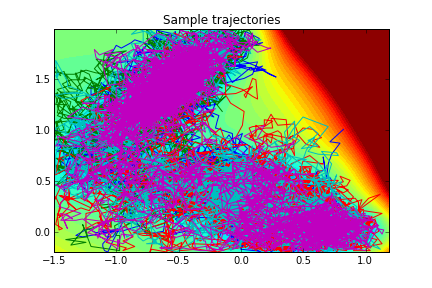
\includegraphics[width=0.8\textwidth]{sample-trajectories.png}
	\caption{5 trajectories of length 250,000 steps}
	\label{sample-trajectories}
\end{figure}


\begin{figure}[htbp!]
	\centering
	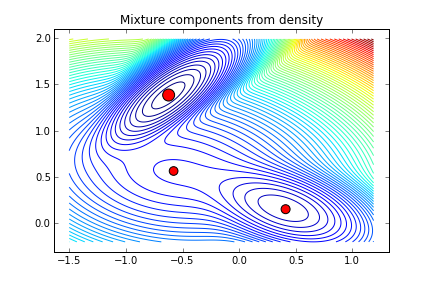
\includegraphics[width=0.8\textwidth]{mix1.png}
	\caption{The initial mixture model without regard
	for the time-series nature of the data. The model
	reflects the lack of density in the transition region.}
	\label{mix1}
\end{figure}

\begin{figure}[htbp!]
	\centering
	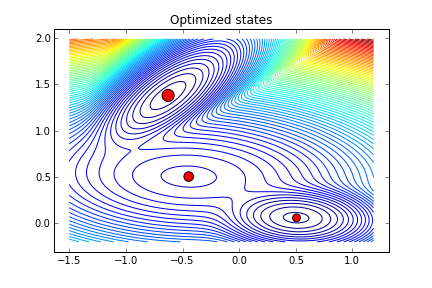
\includegraphics[width=0.8\textwidth]{mix2.png}
	\caption{The optimized hidden states after running the Baum-Welch
	algorithm. Note that this is a sum of three distinct probability distributions,
	each normalized to one.}
	\label{mix2}
\end{figure}

\begin{figure}[htbp!]
	\centering
	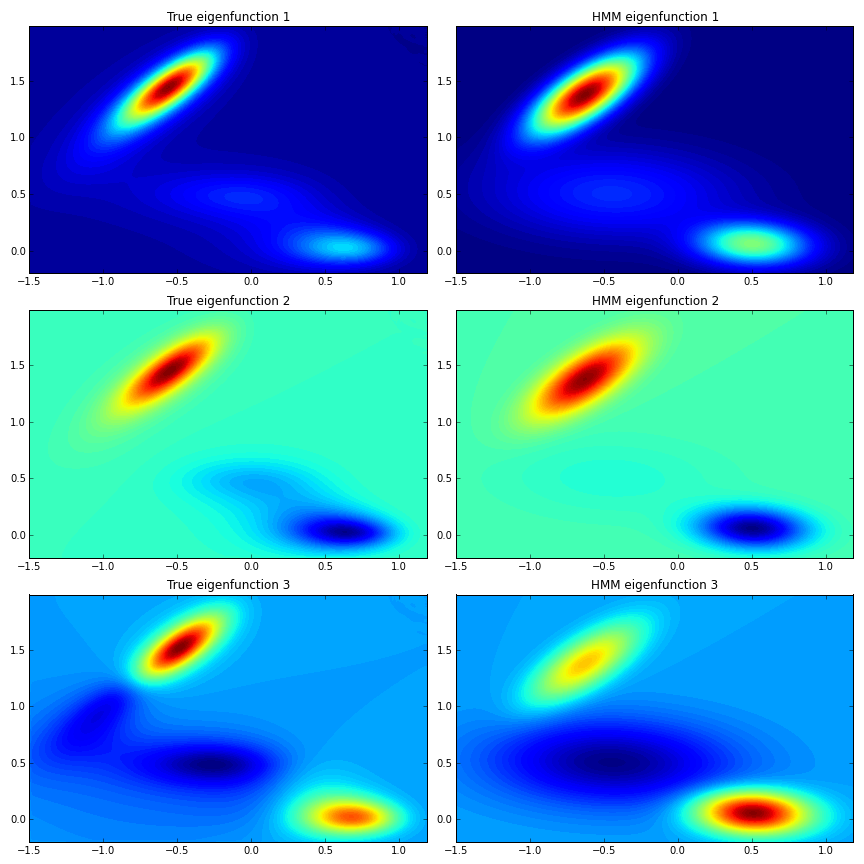
\includegraphics[width=1.0\textwidth]{eigens.png}
	\caption{Visualization of eigenfunctions}
	\label{eigens}
\end{figure}



\subsection{Quantitative Validation}

We hypothesized that HMMs could more accurately predict the implied timescales
(proportional to the eigenvalues of the transition matrix) than a normal
MSM all else being equal. A validation script was run (run tim ~2 days) that performed
HMM and MSM analysis doing all possible permutations of the following parameters:

\begin{itemize}
\item number of clusters($k$): 2 -- 19
\item lag time: 1 -- 29, every two
\item random seed (repeat each case): 10 of them
\end{itemize}

The models were trained on 5 trajectories of length 100,000 steps, strided by 10. For the future,
it would be beneficial to re-do this analysis without striding the data.

\begin{figure}[htbp!]
	\centering
	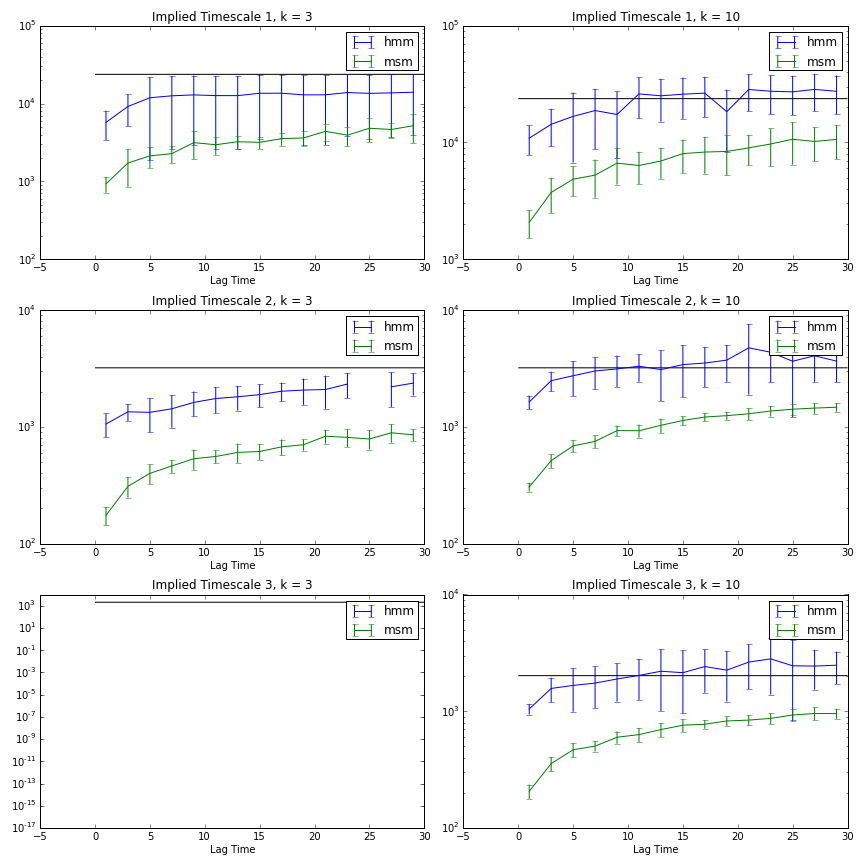
\includegraphics[width=1.0\textwidth]{its_vs_lt.png}
	\caption{Implied timescales vs. lag time.}
	\label{its_vs_lt}
\end{figure}


\begin{figure}[htbp!]
	\centering
	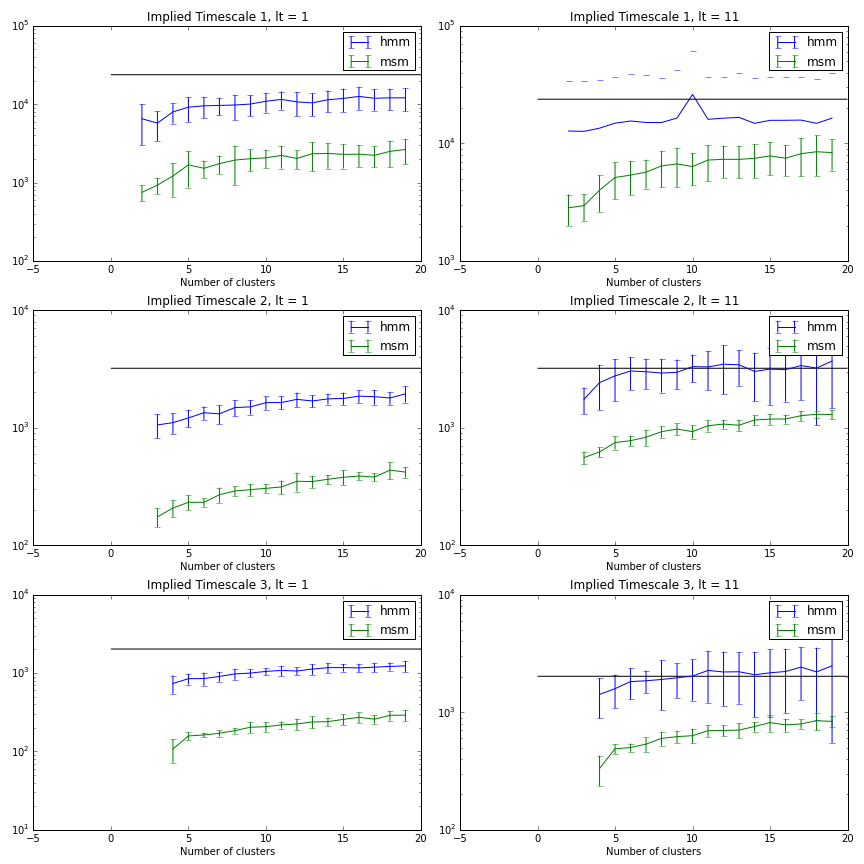
\includegraphics[width=1.0\textwidth]{its_vs_k.png}
	\caption{Implied timescales vs. number of clusters}
	\label{its_vs_k}
\end{figure}

\subsection{Right now}
Re-running with 10 trajectories of 500,000 steps with stride of 5.

Further thoughts: Comparing number of clusters to number of clusters
is kindof unfair. We should use the number of parameters. In MSM, the number
of parameters is just $dim*k$. In the muller potential it is $(dim^2 + dim)*k$.
Using dim=2 and reduce, $k_{msm} = 3*k_{hmm}$. I'm doing this in the new run.

\section{Alanine Dipeptide}
We have applied the HMM model to alanine dipeptide. It is acting fishy.
I would like a better way to visualize the resulting emission distributions;
maybe as ellipses. It is possible that there is one that is just too wide.

The HMM requires that conformations be vectorizable. This is hard to do. I'm suspecting
that using sines and cosines is still messing things up. Those values are confined within
-1 to 1, whereas the emissions use non-wrapping real numbers.

I'm going to try using atom-pair distances.

\end{document}